\section{Introduction}


%%%%%%%%%%%%%%%%%%%%%%%%%%%%%%%%%%%%%%%%%%%%%%%%%%%%%%%%%%%%%%%%%%%%%%%%%%%%%%%
\section{Methodology}

Starting with \citet{Thompson1982} and \citet{Reid1990}, Euler's equation has
been used to estimate the source positions of gravity and magnetic data.
In this section, we will review the solution of Euler's equation for
$(x_o, y_o, z_o)$ by Euler deconvolution \citep{Reid1990} and then present a
new method, called \textit{Euler inversion}, for solving Euler's equation using
total least-squares.

We start with Euler's homogeneity equation

\begin{equation}
  (x - x_o)\partial_x f + (y - y_o)\partial_y f + (z - z_o)\partial_z f
  + \eta(f - b) = 0
  \ ,
  \label{eq:euler}
\end{equation}

\noindent
in which $f$ is a homogeneous function (in this case, a potential-field),
$(x, y, z)$ are the coordinates of the observation point,
$(x_o, y_o, z_o)$ are the coordinates of the field source,
$b$ is the base level representing a constant shift in the field,
and $\eta$ is the structural index, which is related to the nature of the
source and how its potential-field values decay with distance \citep{Reid2014}.
Equation~\ref{eq:euler} relates the coordinates of the source with the observed
potential field and its gradient.

Given $N$ observations points in which we have measured $f$ and its gradient
(for a total $4N$ data), both Euler deconvolution and Euler inversion aim to
estimate the parameter vector

\begin{equation}
  \mathbf{p} = \begin{bmatrix}x_o & y_o & z_o & b \end{bmatrix}^T.
  \label{eq:p}
\end{equation}

\subsection{Euler deconvolution}

Euler deconvolution starts by rearranging Equation~\ref{eq:euler} to place the
parameters on the left-hand side and all other terms on the right-hand side,
forming an $N \times 4$ equation system

\begin{equation}
  \begin{aligned}
  -x_o\partial_x f_1 - y_o\partial_y f_1 - z_o\partial_z f_1 - \eta b &= -x_1\partial_x f_1 - y_1\partial_y f_1 - z_1\partial_z f_1 - \eta f_1
  \\
  -x_o\partial_x f_2 - y_o\partial_y f_2 - z_o\partial_z f_2 - \eta b &= -x_2\partial_x f_2 - y_2\partial_y f_2 - z_2\partial_z f_2 - \eta f_2
  \\
  \vdots
  \\
  -x_o\partial_x f_N - y_o\partial_y f_N - z_o\partial_z f_N - \eta b &= -x_N\partial_x f_N - y_N\partial_y f_N - z_N\partial_z f_N - \eta f_N
  \end{aligned}
  \ ,
\end{equation}

\noindent
which can be written in matrix form as

\begin{equation}
  \underbrace{
    \begin{bmatrix}
      -\partial_x f_1 & -\partial_y f_1 & -\partial_z f_1 & -\eta \\
      -\partial_x f_2 & -\partial_y f_2 & -\partial_z f_2 & -\eta \\
      \vdots & \vdots & \vdots & \vdots \\
      -\partial_x f_N & -\partial_y f_N & -\partial_z f_N & -\eta
    \end{bmatrix}
  }_{\mathbf{A}}
  \underbrace{
    \begin{bmatrix}
      x_o \\ y_o \\ z_o \\ b
    \end{bmatrix}
  }_{\mathbf{p}}
  =
  \underbrace{
    \begin{bmatrix}
      -x_1\partial_x f_1 - y_1\partial_y f_1 - z_1\partial_z f_1 - \eta f_1 \\
      -x_2\partial_x f_2 - y_2\partial_y f_2 - z_2\partial_z f_2 - \eta f_2 \\
      \vdots \\
      -x_N\partial_x f_N - y_N\partial_y f_N - z_N\partial_z f_N - \eta f_N \\
    \end{bmatrix}
  }_{\mathbf{c}}
  \ ,
  \label{eq:deconv-system}
\end{equation}

\noindent
in which $\mathbf{A}$ is the Jacobian matrix of Euler's equation
(Equation~\ref{eq:euler}) with respect to the parameters
(Equations~\ref{eq:p})
and $\mathbf{c}$ is a \textit{pseudo-data vector}.

The solution proposed by \citet{Thompson1982} and \citet{Reid1990} is a
least-squares estimate of $\mathbf{p}$

\begin{equation}
  \hat{\mathbf{p}} = \left(\mathbf{A}^T\mathbf{A}\right)^{-1}
  \mathbf{A}^T\mathbf{c}
  \ .
  \label{eq:deconv-p}
\end{equation}

\noindent
However, the solution above is valid only if the contents of the Jacobian
matrix $\mathbf{A}$ are assumed to be error-free.
As can be seen from Equation~\ref{eq:deconv-system}, the Jacobian contains the
derivatives of $f$, which are often computed numerically by finite-differences
or Fourier transforms and are known to amplify the high-frequency random noise
in the data.
This presents a problem, particularly for the estimation of $z_o$, which has
been widely explored in the literature [CITATION NEEDED].


\subsection{Euler inversion}


Starting values for p and d.

\subsection{Estimating the structural index}

\subsection{Windowing procedure}


%%%%%%%%%%%%%%%%%%%%%%%%%%%%%%%%%%%%%%%%%%%%%%%%%%%%%%%%%%%%%%%%%%%%%%%%%%%%%%%
\section{Results}


\subsection{Method demonstration with a single window}

\begin{figure}[tb!]
\centering
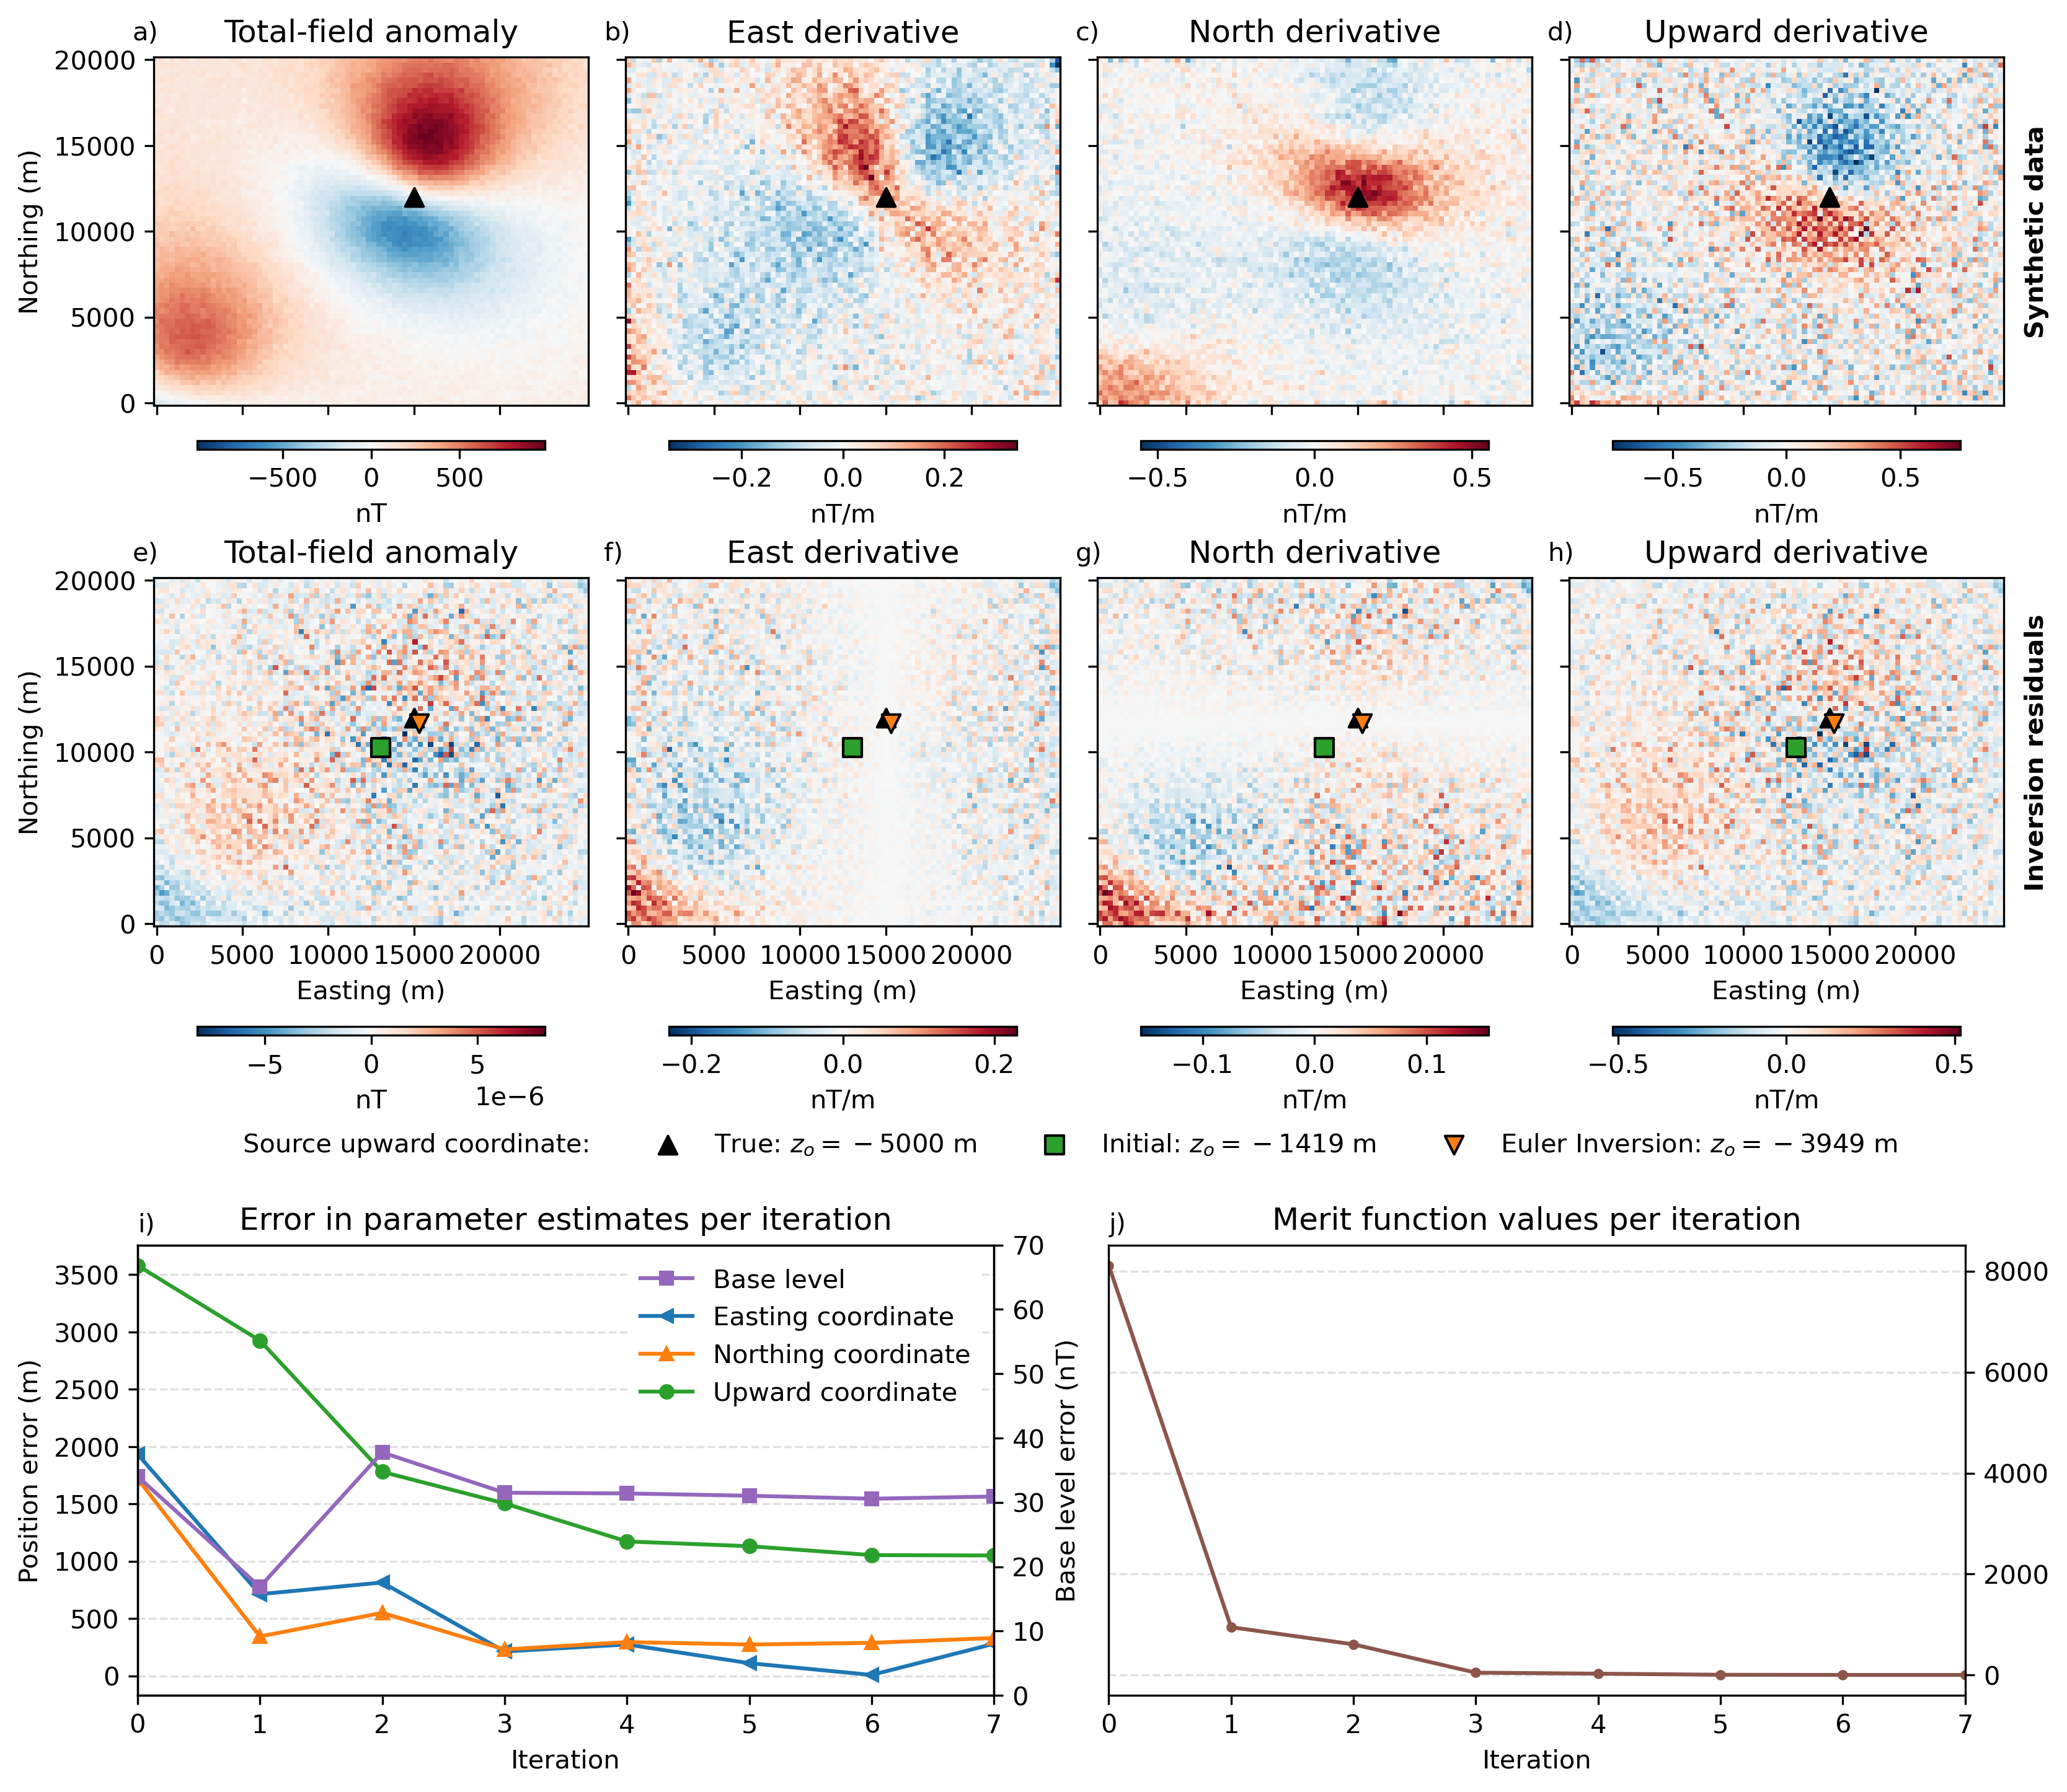
\includegraphics[width=1\linewidth]{figures/synthetic-proof-of-concept.png}
\caption{
  \lipsum[1]
}
\label{fig:proof}
\end{figure}


\subsection{Effect of random noise}

\begin{figure}[tb!]
\centering
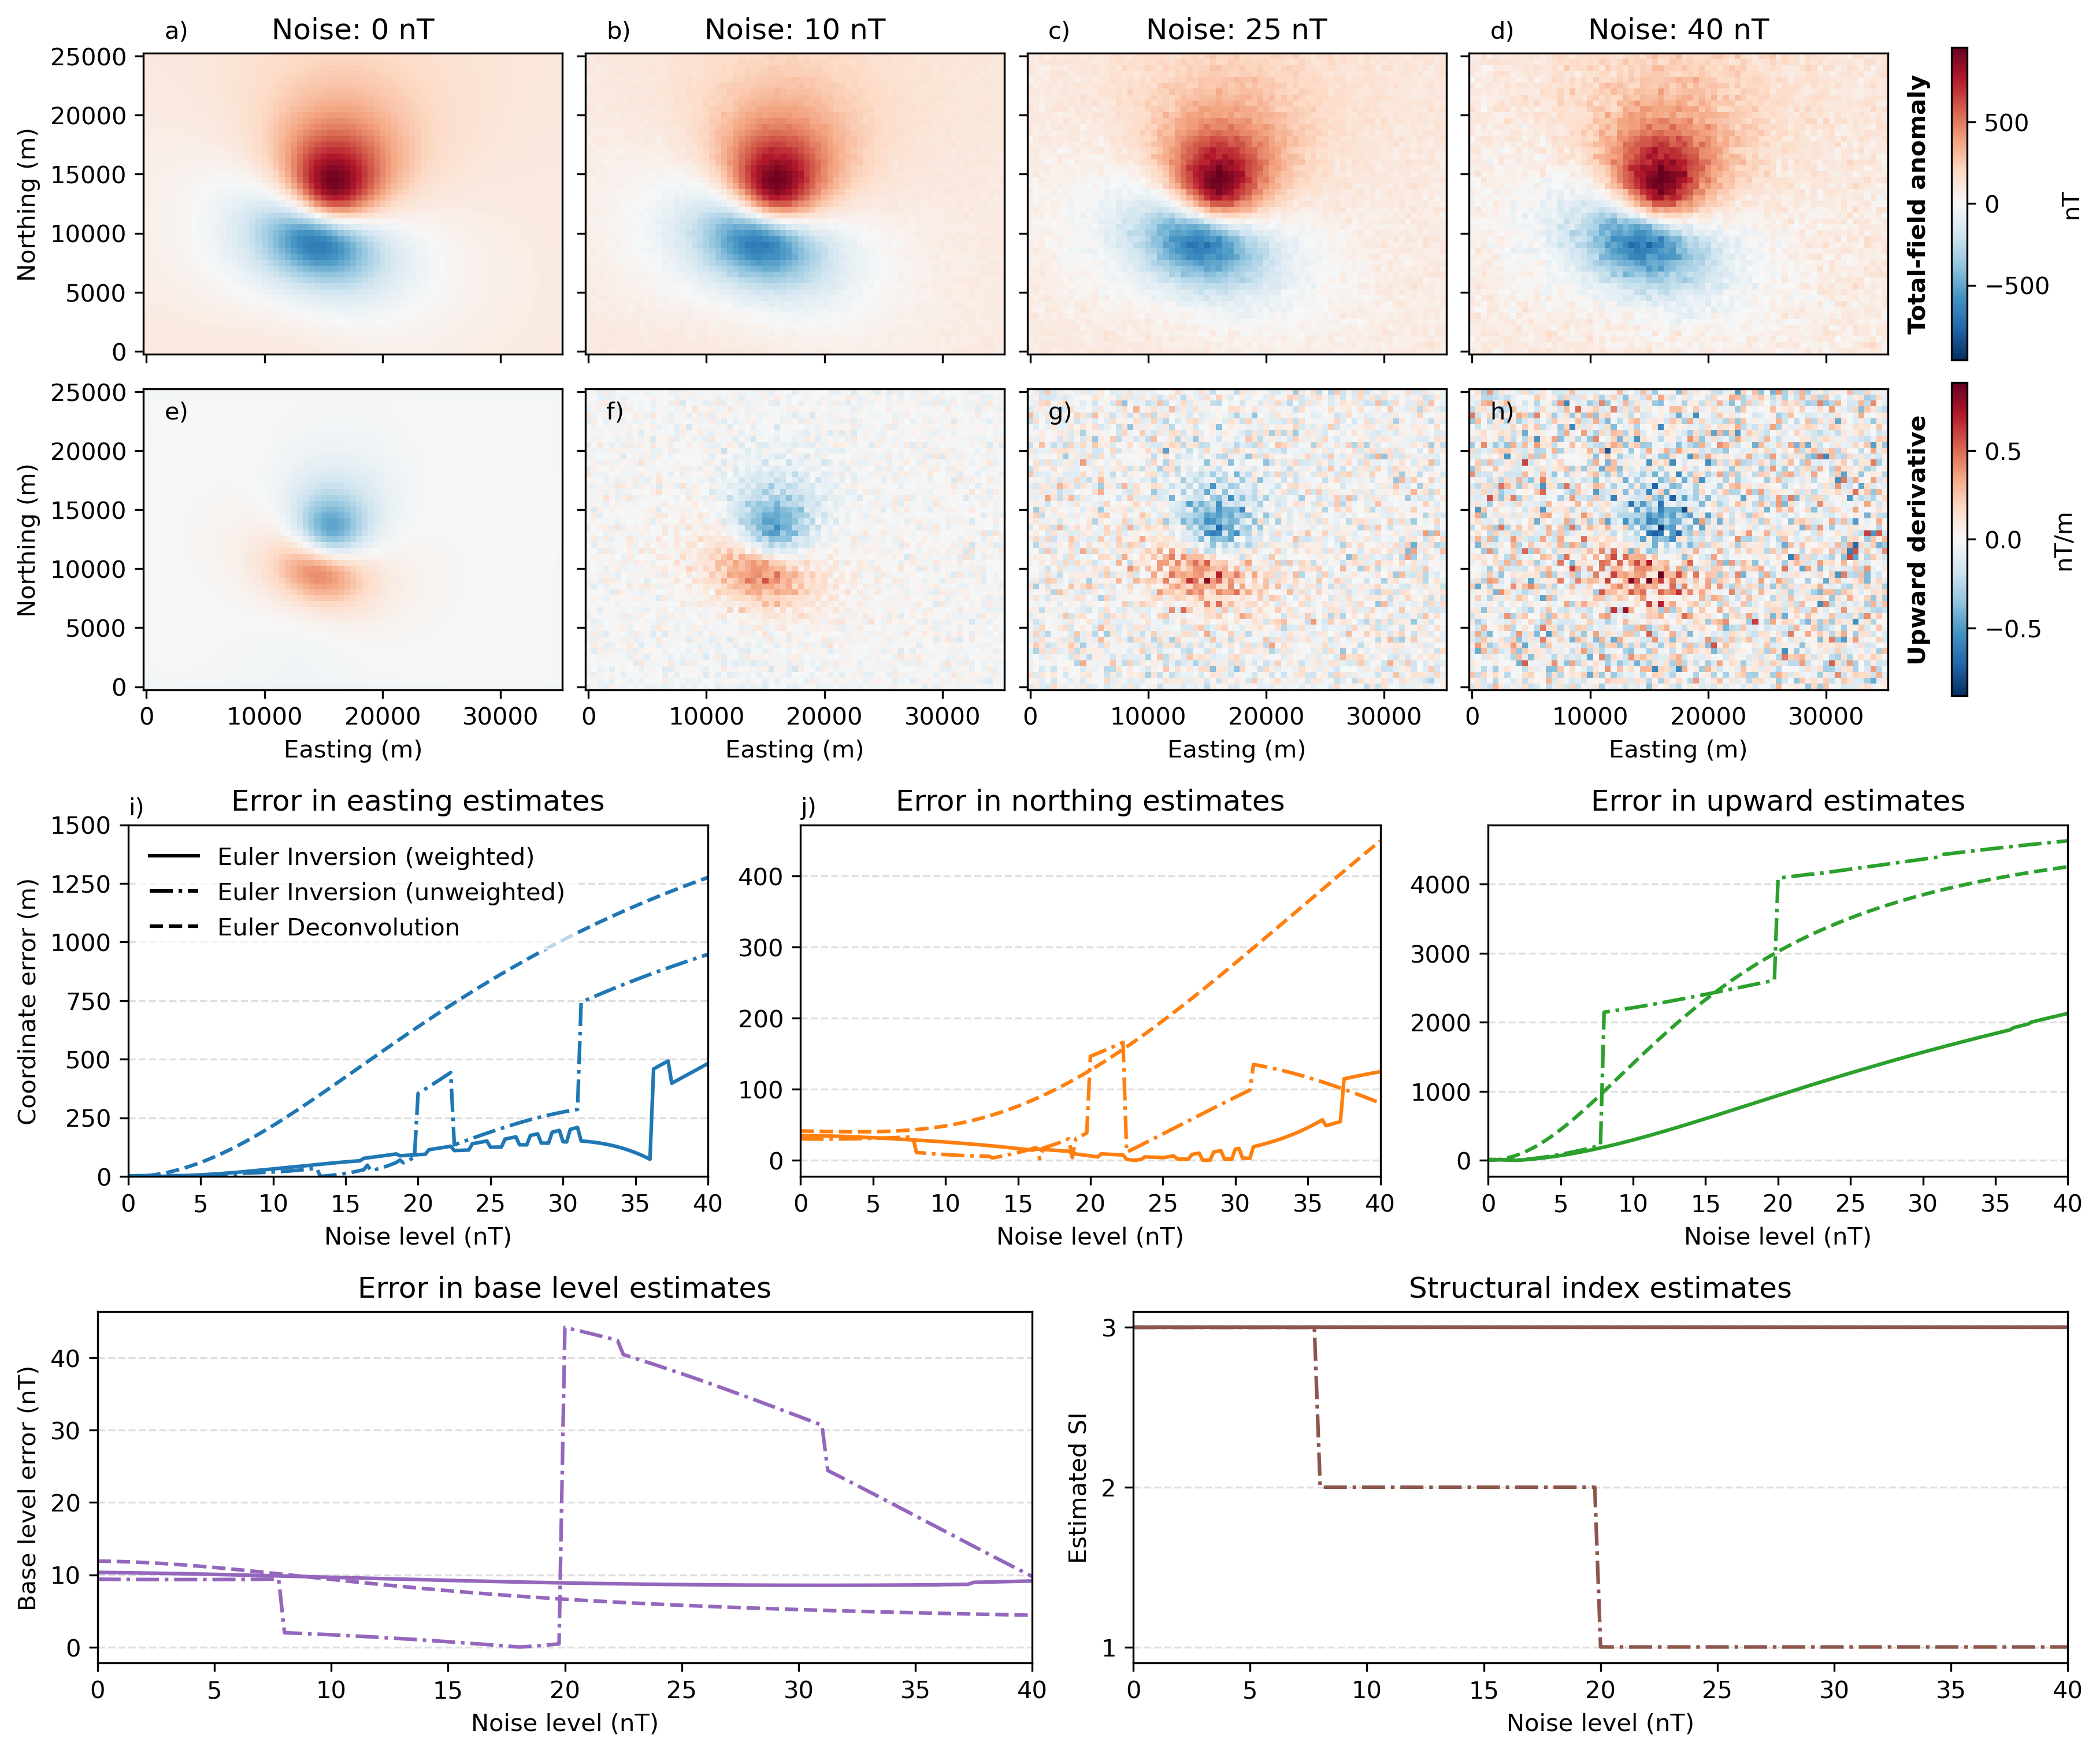
\includegraphics[width=1\linewidth]{figures/synthetic-noise-levels.png}
\caption{
  \lipsum[1]
}
\label{fig:noise}
\end{figure}

\subsection{Effect of SI on multiple sources}

\begin{figure}[tb!]
\centering
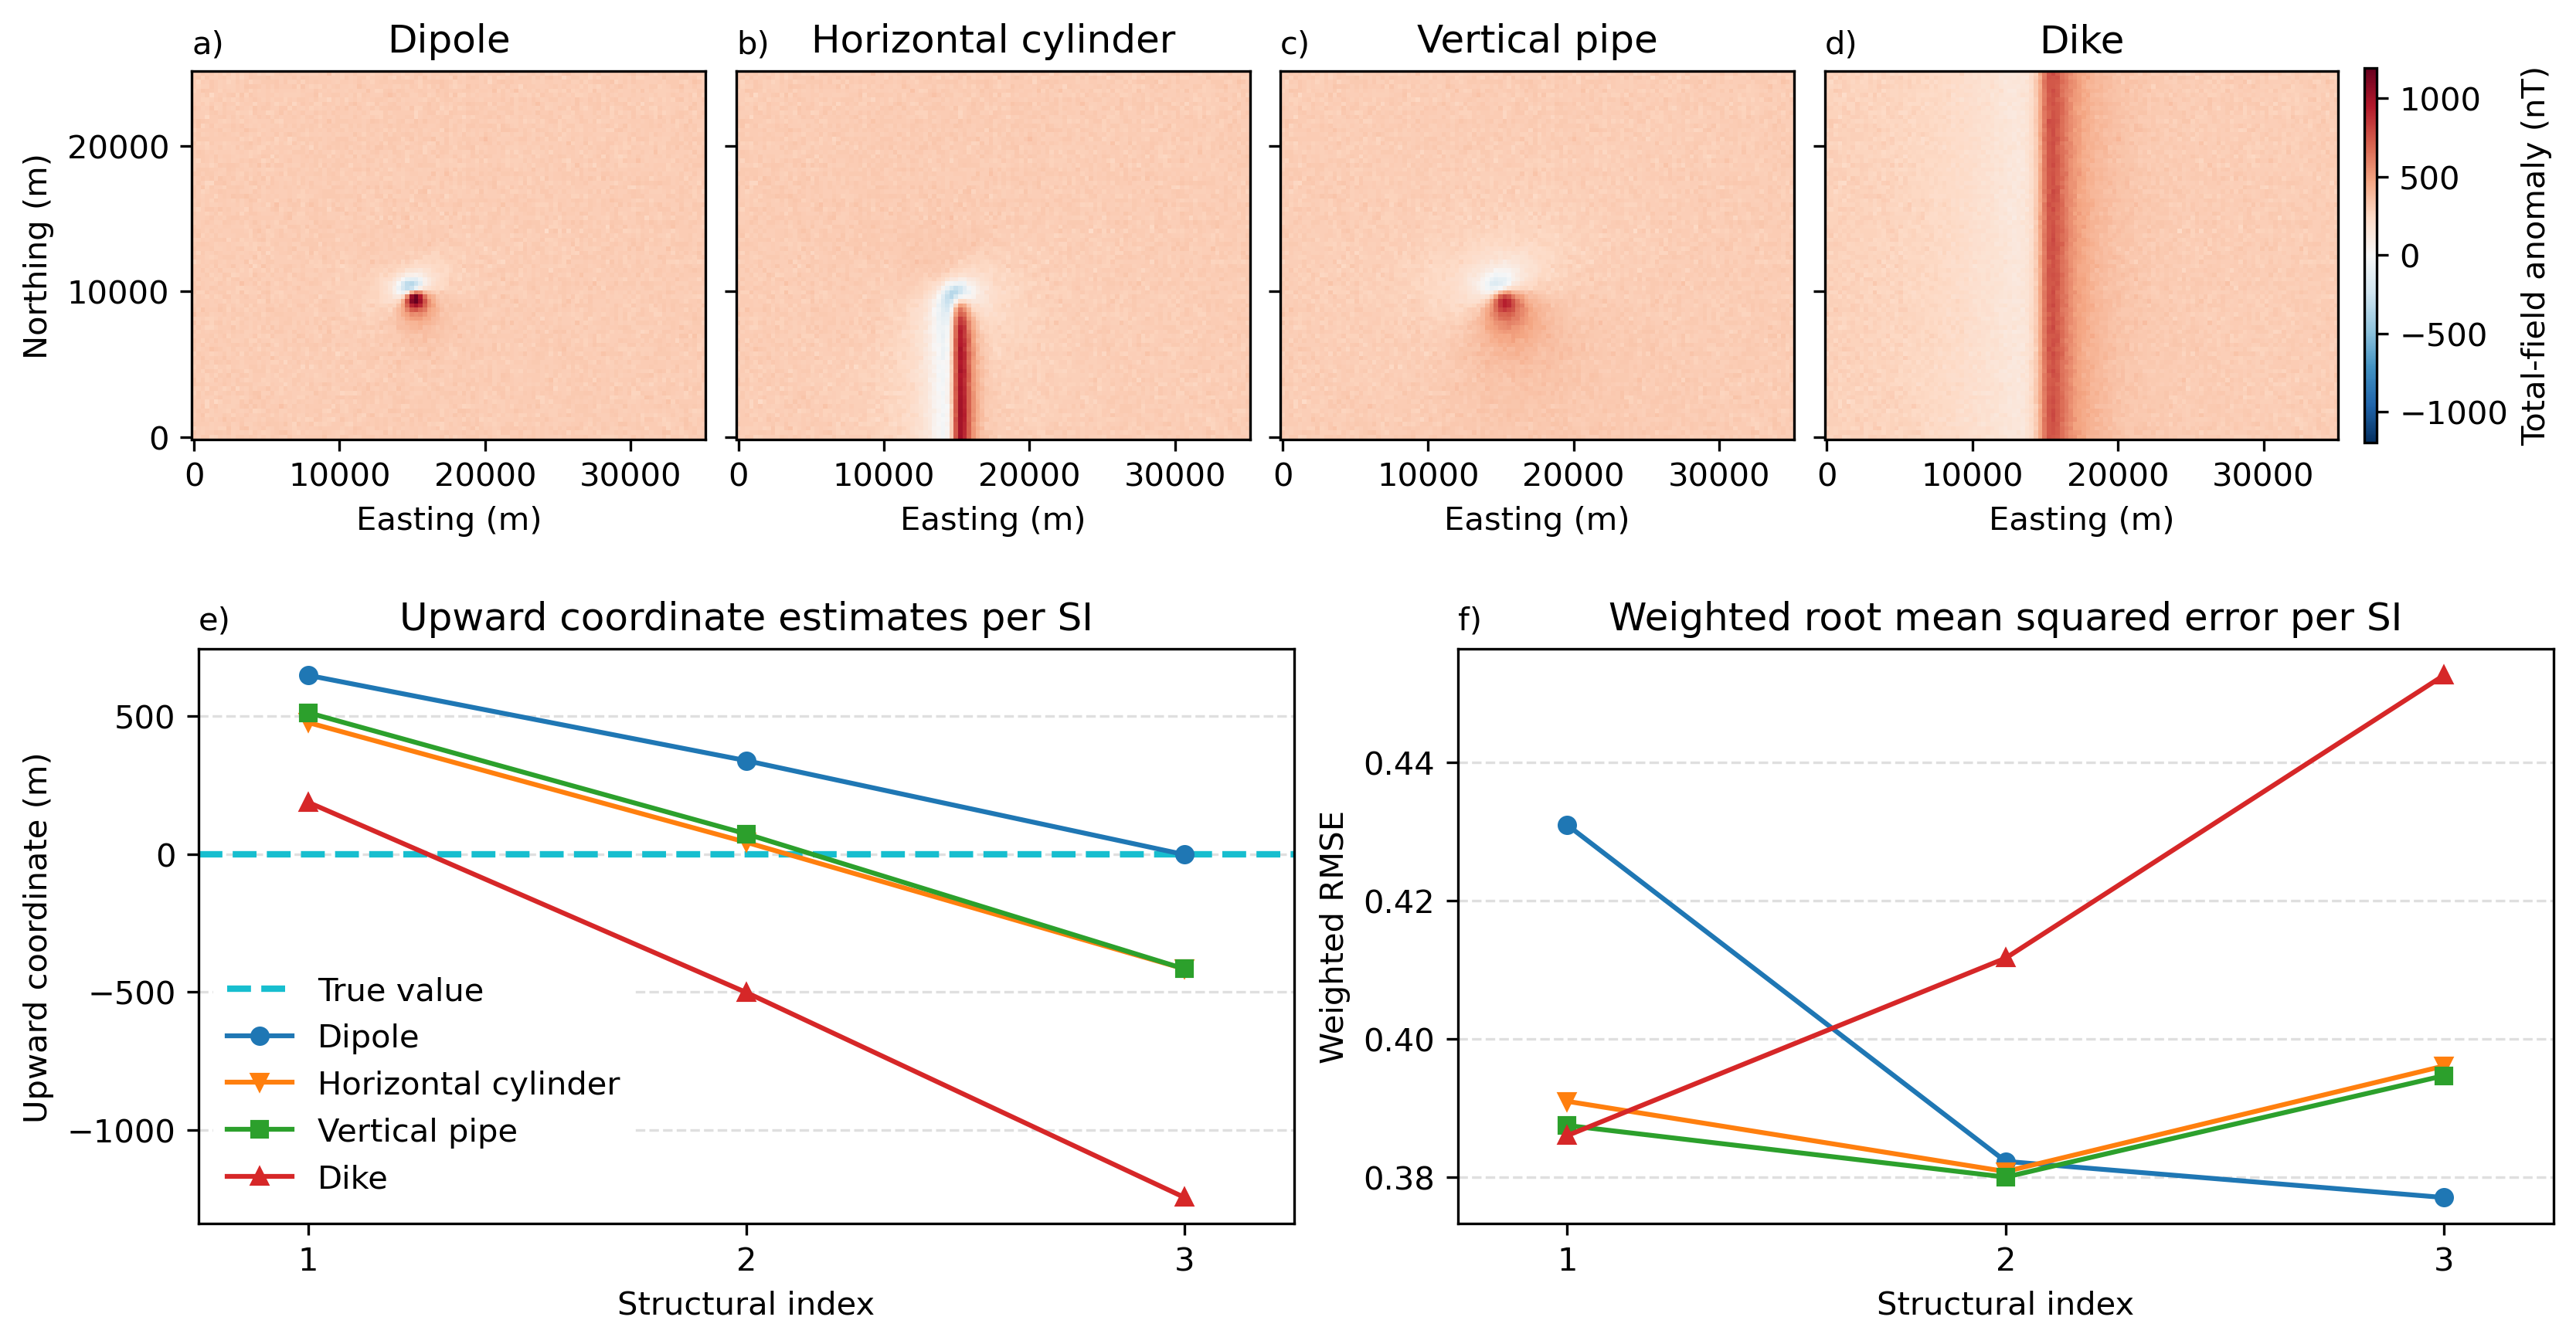
\includegraphics[width=1\linewidth]{figures/synthetic-structural-index.png}
\caption{
  \lipsum[1]
}
\label{fig:si}
\end{figure}

\subsection{Windowing procedure with multiple sources}

\begin{figure}[tb!]
\centering
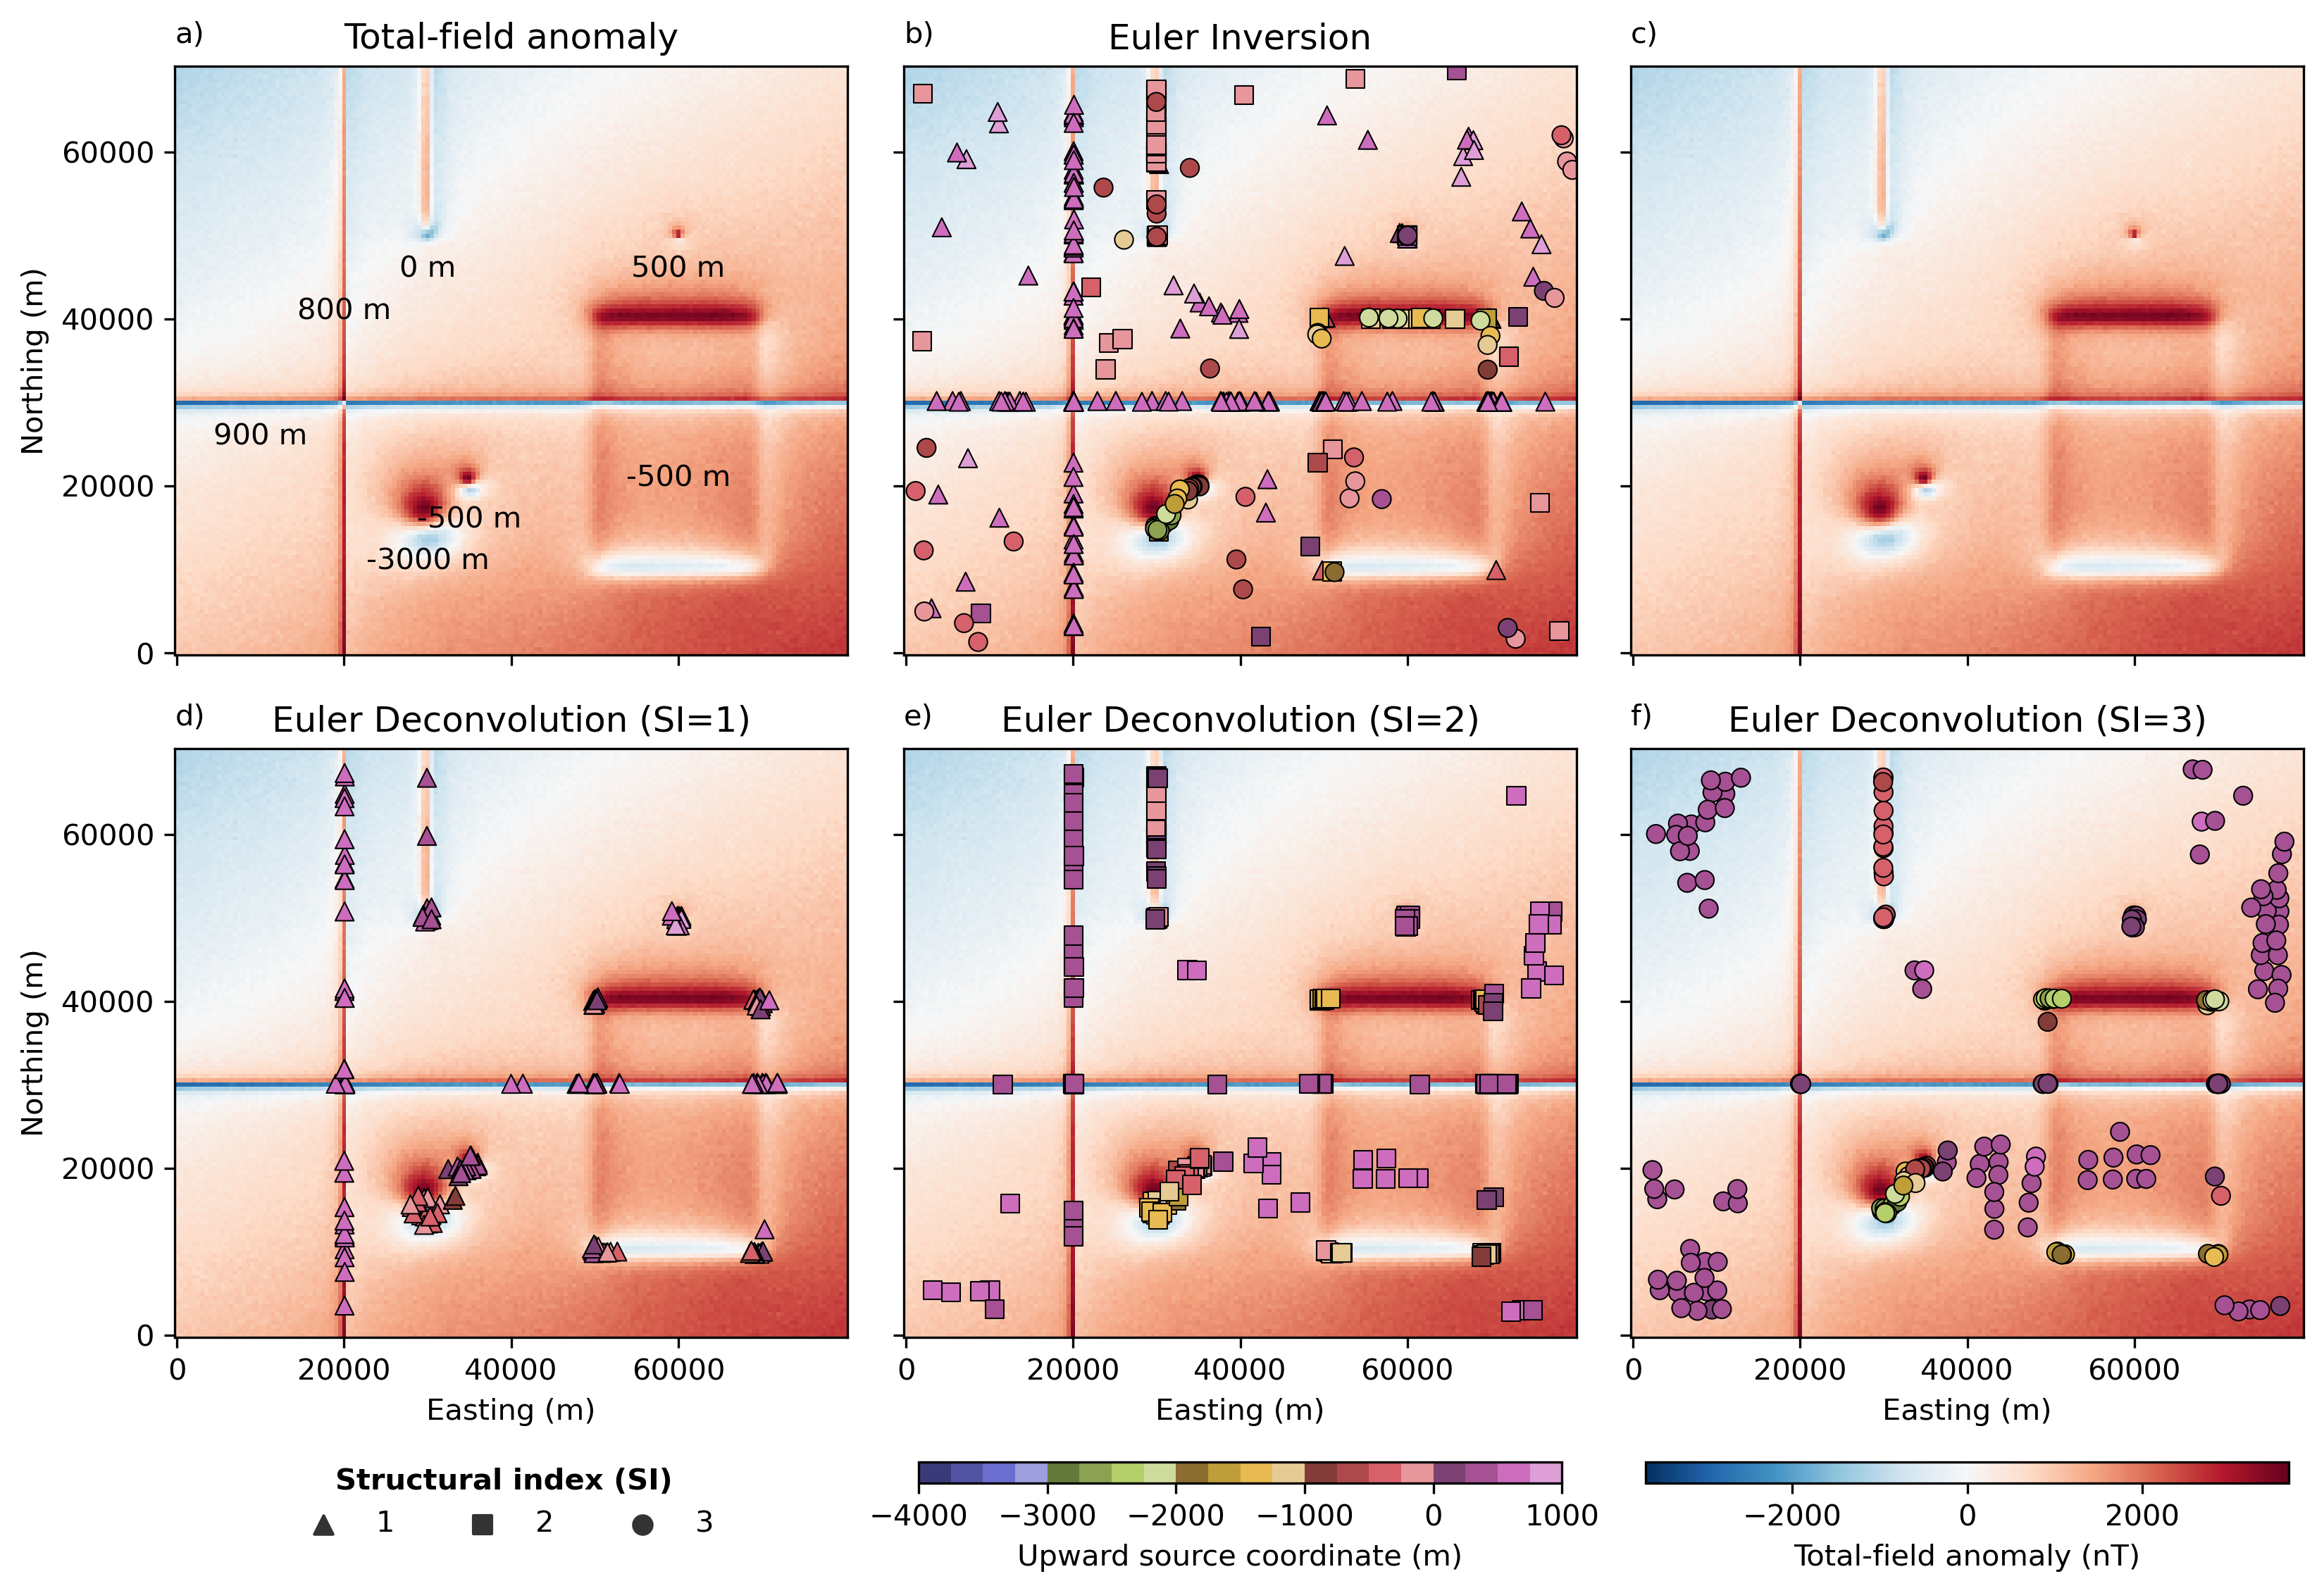
\includegraphics[width=1\linewidth]{figures/synthetic-windows.png}
\caption{
  \lipsum[1]
}
\label{fig:windows}
\end{figure}

\subsection{Aeromagnetic data from Rio de Janeiro}

%%%%%%%%%%%%%%%%%%%%%%%%%%%%%%%%%%%%%%%%%%%%%%%%%%%%%%%%%%%%%%%%%%%%%%%%%%%%%%%
\section{Conclusion}



%%%%%%%%%%%%%%%%%%%%%%%%%%%%%%%%%%%%%%%%%%%%%%%%%%%%%%%%%%%%%%%%%%%%%%%%%%%%%%%
\section{Open research}

The Python source code used to produce all results and figures presented here
is available at \url{https://github.com/\GitHubRepository} and
\url{https://doi.org/\ArchiveDOI} under the MIT open-source license.

Here we should cite all of the main software used, like Jupyter, numpy, scipy,
matplotlib, Fatiando, etc.

Cite any data sources as well.



%%%%%%%%%%%%%%%%%%%%%%%%%%%%%%%%%%%%%%%%%%%%%%%%%%%%%%%%%%%%%%%%%%%%%%%%%%%%%%%
\section{Acknowledgements}

We are indebted to the developers and maintainers of the open-source software
without which this work would not have been possible.
Acknowledge any non-author contributors to this study.
Statement about funding.

% Thank the editors and reviewers after review.
